\documentclass{article}
\usepackage{tikz}
\usepackage{amsmath}
\usepackage{amssymb}
\usepackage{pgfplots}
\usepackage{amsthm}
\usepackage{cancel}
\pgfplotsset{compat=1.16}
\usetikzlibrary{calc}
\title{Matrix Lie Groups}

\newtheorem*{remark}{Rotation Criterion}

\begin{document}
\author{Thomas Brown}
\maketitle


\section{Introduction to Lie Theory}
Matrix Lie groups are algebraic structures that generalize the familiar physical symmetries of space, and include for example space rotations. These rotations are represented by matrices that transform a basis vector (the group identity) to another matrix in the group. The set of all such transformations constitutes the Lie group. Operations in the Lie algebra observe certain properties that constitute being a 'smooth manifold' which, in the simpler context of matrix Lie groups, means that every Ax generates a rotation in the group: \[A \in \mathfrak{g}, g \in G \implies gAg^{-1} \in \mathfrak{g}\]

\section{The Trivial $\mathbb{S}^1$ Group}
$\mathbb{S}^1$ is the set generated through angle $\theta$ in the complex plane $e^{i\theta}$ = $cos\theta + isin\theta$. \begin{center}$\mathbb{S}^1$ = $\left\{ z \in \mathbb{R}^2 : |z| = 1 \right\}$ \end{center}
The elements in $\mathbb{S}^1$ constitute a commutative group, which makes the application of Lie Theory trivial. Matrices are used to represent complex numbers because they behave exactly the same under multiplication and addition. This is easy to see if we represent each rotation $R_{\theta}$ as a linear combination of the basis matrices:\[
R_{\theta} = cos{\theta}\begin{pmatrix}1 & 0 \\0 & 1\end{pmatrix}
+ sin{\theta}\begin{pmatrix}0 & -1\\1 & 0\end{pmatrix}
\]
It is easily checked that the matrix representing $\sqrt{-1}$ is exactly the same as $\mathfrak{i}$
\[
i^2 = \begin{pmatrix}0 & -1\\1 & 0\end{pmatrix}^2 = -1
\]
Here we have written "-1" for the negative of the 2x2 identity matrix.
    The exponentiation of the vector $i\theta$ is a key idea that allows you to map the Lie algebra space onto the manifold. The opposite map is called the logarithm map which forms the basis for operations of elements in the Lie algebra.
The same calculation can be made for the identity matrix.
To delve into higher dimensional groups, it is easier to visualize the $\mathbb{S}^1$ group and its corresponding Lie algebra in a coordinate system. 
\begin{center}
\begin{tikzpicture}[scale=3]
    % Draw the unit circle
    \draw[thick] (0,0) circle (1cm);
    \draw[->, thick, blue] (1,0) arc (0:60:1) node[above right] {$e^{i\theta}$};
    % Draw the axes
    \draw[->] (-1.2,0) -- (1.2,0) node[right] {$\Re$};
    \draw[->] (0,-1.2) -- (0,1.2) node[above] {$\Im$};
    
    % Draw the tangent vector
    \draw[->,red] (1,0) -- (1,1) node[midway, above right] {$i\theta$};
    
    % Draw the point (1,0)
    \filldraw (1,0) circle (1pt) node[below right] {1};
\end{tikzpicture}
\end{center}
The tangent vector at the identity point (1,0) spans the Lie algebra of $\mathbb{S}^1$ and the unit circle is the group $\mathbb{S}^1$ itself. The tangent vector's magnitude can be thought of in terms of the velocity at that point, where some rotation can move the vector along the length of the circle. The notion of an infinitesimal change in such a rotation will be important later on when we discuss operations in the Lie Algebra. For now, we can entertain a simpler description of a manifold in terms of the $\mathbb{S}^1$ group. If we zoom in on any point of the unit circle, we can see that the local neighborhood around the point can be smoothly deformed into a straight line and that line can be deformed back into an arc. Extending this definition to a group of higher dimensional rotations, such as the result of the Cartesian product of $\mathbb{S}^1$ with itself (a torus):
\[
\mathbb{S}^1 \times \mathbb{S}^1 = \{(z_1, z_2) : z_1, z_2 \in S^1 \}
\]
The local neighborhood around the identity no longer resembles a line, but a plane, so it is a 2-dimensional manifold.

\section{The Groups $SO(3)$ and $SU(2)$}
The group $SO(2)$ of rotations about $O$ can be viewed as the unit circle ($\mathbb{S}^1$) as demonstrated above. The 2-sphere $\mathbb{S^2}$ is not a Lie group since there is no product rule that makes it a group. We can construct the $\mathbb{S}^3$ group with unit quaternions and represent them with complex matrices since, in general, they are both non-commutative. \[
Q = \begin{pmatrix}a+di & -b-ci\\b-ci & a-di\end{pmatrix} , det(Q) = 1
\]
The set of 2x2 complex matrices with this determinant condition form the special unitary group $SU(2)$. Since $SU(2)$ is a Lie group, observations can be made about it in group theory.
Take the quaternion $t = sin\theta + ucos\theta$ where u is a unit quaternion. Then conjugation of any unit quaternion $q \in SU(2)$ by t induces a homomorphism $\phi : q \mapsto tqt^{-1}$. The $SO(3)$ group operation corresponds to quaternion multiplication by the rule \[(\pm t_{1})(\pm t_{2}) = (\pm t_{1}t_{2})\]
We can construct a map from the unit quaternions t and -t to the antipodal pair $\pm t$ in $SO(3)$. Since each unit t and -t is mapped to a single pair in $SO(3)$, $SO(3)$ is a quotient of $SU(2)$. The map's kernel $ker(\phi)$ = $\{1,-1\}$ has 2 elements so this is a 2-1 homomorphism of groups.

\section{Lie Algebra of SO(3)}
The Lie Algebra of $SO(3)$, denoted by the lowercase fraktur font $\mathfrak{so}(3)$, can be studied using a manifold view or a vector space view. One may be easier to use depending on the property we want to prove or interpret. For the purpose of this reading, we will use the manifold view since it is readily visualizable.
\[\]
\begin{center}
    Below is the depicted 3-D manifold of $SO(3)$
\end{center}
\begin{minipage}{0.55\textwidth}
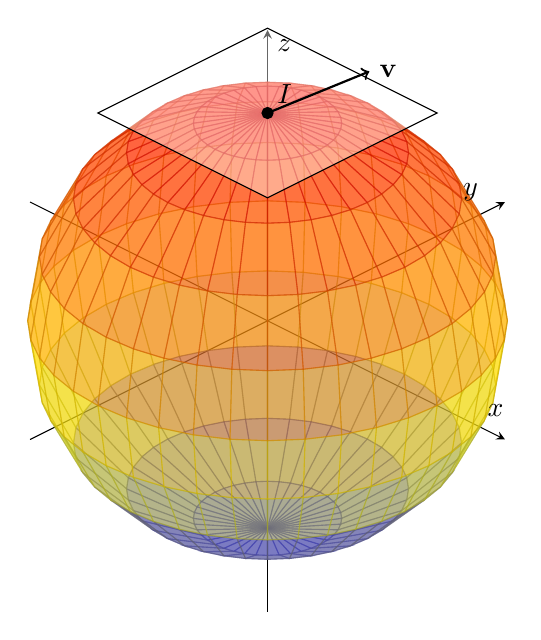
\begin{tikzpicture}[tangent plane/.style args={at #1 with vectors #2 and #3}{%
insert path={#1 --  ($#1+($#2-(0,0,0)$)$) --  ($#1+($#2-(0,0,0)$)+($#3-(0,0,0)$)$) 
-- ($#1+($#3-(0,0,0)$)$) -- cycle}}]
    \begin{axis}[%
        axis equal,
        width=15cm,
        height=15cm,
        axis lines = center,
        xlabel = {$x$},
        ylabel = {$y$},
        zlabel = {$z$},
        ticks=none,
        enlargelimits=0.2,
        view/h=45,
        scale uniformly strategy=units only,
    ]
    \addplot3[%
        opacity = 0.5,
        surf,
        z buffer = sort,
        samples = 21,
        variable = \u,
        variable y = \v,
        domain = 0:180,
        y domain = 0:360,]
    ({cos(u)*sin(v)}, {sin(u)*sin(v)}, {cos(v)});
    \draw[fill=white,fill opacity=0.4,
    tangent plane=at {(-0.5,-0.5,1)} with vectors {(1,0,0)} and {(0,1,0)}];
    % Vector with magnitude 1
    \draw[->, thick] (0,0,1) -- (0.3,0.3,1.2) node[right] {$\mathbf{v}$};
    \filldraw (0,0,1) circle (2pt) node[above right] {$I$};
    \end{axis}
\end{tikzpicture}
\end{minipage}
 \footnote{Note that this diagram is for illustrative use only and does not represent the actual SO(3) group}
\begin{minipage}{0.55\linewidth}
    Referring back to our example with the unit circle, we can see that the Lie Algebra was a 1-dimensional line. Assuming an anti-clockwise rotation, the corresponding vectors for (0,1) and (1,0) can be denoted as 
    \[\begin{pmatrix}0\\a\end{pmatrix} \begin{pmatrix}-a\\0\end{pmatrix}\]
    This yields the following set of matrices for $\mathfrak{so}(2)$: 
    \[\mathfrak{so}(2) = \{\begin{pmatrix}0&a\\-a&0\end{pmatrix} : a \in \mathbb{R}\}\]
    The same construction can be used for the Lie Algebra of $\mathfrak{so}(3)$. Starting with the vector $v$ displayed, we see that it is on the plane $z=1$, so its corresponding vectors for (0,0,1), (0,1,0) and (0,0,1) would be $\begin{pmatrix}0\\a\\b\end{pmatrix}$$\begin{pmatrix}c\\0\\d\end{pmatrix}$$\begin{pmatrix}e\\f\\0\end{pmatrix}$
\end{minipage}
The resulting matrix $\begin{pmatrix}0&a&b\\c&0&d\\e&f&0\end{pmatrix}$ with columns corresponding to the velocities of those points. However, not every matrix represents a rotation in $SO(n)$. Below is a definition:
\begin{remark}
    A $n\times n$ matrix $R$ represents a rotation in SO(n) if and only if $RR^{T} = I$ and $det(R) = 1$.
\end{remark}
We can contextualize this with some simple calculations accurate up to O($\epsilon$) \[RR^{T} = I\]
\[\implies(I + \epsilon A)^{T}(I + \epsilon A) = I\]
\[\implies I + \epsilon(A + A^{T}) + \cancel{\epsilon^{2}AA^{T}} = I\]
\[\implies A^{T} = -A\]
If A is to be in the Lie Algebra, then it must be anti-symmetric.
\[A \in \mathfrak{so}(n) \implies A^{T} = -A\]
In addition to the orthogonality condition, $R$ must also be orientation preserving, hence the determinant condition.

\section{Simple Properties of the Lie Algebra}
We've noted 2 simple properties of the Lie Algebra: It is a vector space and\[ A \in \mathfrak{g},g \in G \implies gAg^{-1} \in \mathfrak{g}.\]
The first property is easy to see taking the "manifold view" since any n vectors tangent to the identity will span the space $\mathbb{R}^{n-1}$.
In the vector view, however, demonstrating this is a bit more involved.

Let Ax, Bx be vector fields that generate rotations in SO(3). For a general point x, follow Bx for a short time $\epsilon$. The new position of x is then $(I + \epsilon B)x$ (accurate up to $O(\epsilon))$, then follow Ax for time $\epsilon$. The total displacement will be the effect of the $(I + \epsilon B)(I + \epsilon A)x - x$.

Canceling out the higher terms, we arrive at $\epsilon(A+B)x$. The velocity is then 
\[\longrightarrow\frac{\epsilon(A+B)x}{2\epsilon} \]
\[\longrightarrow (\frac{A+B}{2})x\] 
\[\longrightarrow (A+B)x\] 
Therefore (A+B)x generates a rotation in $SO(3)$.
The second property has to do with the crude definition of a "smooth manifold" provided in the introduction and in order to visualize it we must take an infinitesimal look at intermediate transformations between A and $gAg^{-1}$.

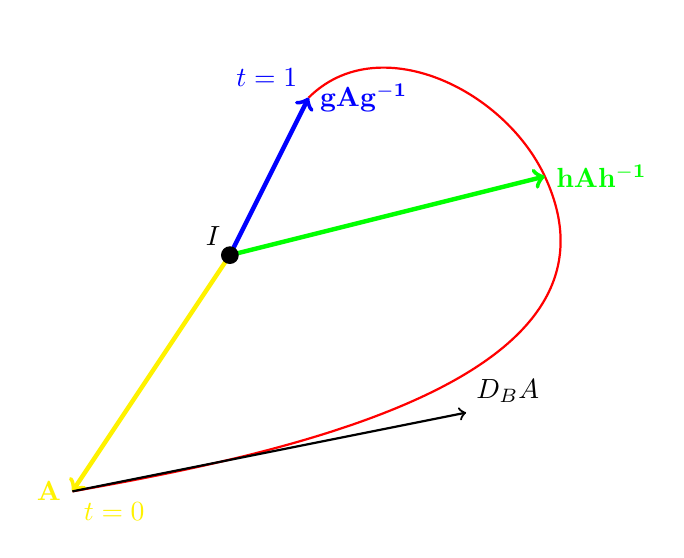
\begin{tikzpicture}
    \draw [thick,red] (-2,2) to[out=45,in=115] (1,1) to[out=-180+115,in=10] (-5,-3);
    \draw[->,ultra thick,blue](-3,0) -- (-2,2) node[right] {$\mathbf{gAg^{-1}}$} node[above left] {$t=1$};
    \draw[->,ultra thick,yellow](-3,0) -- (-5,-3) node[left] {$\mathbf{A}$} node[below right] {$t=0$};
    \draw[->,ultra thick,green](-3,0) -- (1,1) node[right]{$\mathbf{hAh^{-1}}$};
    \filldraw (-3,0) circle (3pt) node[above left] {$I$};
    \draw[->,thick,black] (-5,-3) -- (0,-2) node[above right] {$D_{B}A$};
\end{tikzpicture}

The exponential map $e^{B}$ generates a rotation in the Lie group, so the intermediate transformations can be represented as a function $f(t)$ =  $e^{tB}Ae^{-tB}$ for some time t. To study the properties of the infinitesimal transformation, we can derive $f^{'}(0)$ as such
\[f^{'}(0) = \lim_{t\to 0}{\frac{e^{tB}Ae^{-tB}-A}{t}}\]
\[= \lim_{t\to 0}{\frac{1}{t}((1+tB)A(1-tB)-A)}\]
cancelling out higher order terms, we arrive at
\[= \lim_{t\to 0}{\frac{1}{t}(A+t(BA-AB)-A)}\]
\[= BA-AB\]
The result can be thought of as the derivative of A in the direction of B,  denoted in the diagram as $D_{B}A$, or as $ad_{B}A$ in traditional notation. The key idea is that this derivative exists at every point in the path taken to a transformation.

\section{Properties of the adjoint}
We recovered the following definition of the adjoint in terms of the directional derivative at a point $ad_{B}A$ = BA - AB. The first property we want to show is alternativity: \[ad_{A}A = 0\]
If you have a vector field Ax and rotate it using a rotation generated by A, then you still end up with the same vector field Ax. So the rate of change of the vector field is 0 since it hasn't changed.
The second property is bilinearity: \[
ad_{A}(\lambda B_{1} + \mu B_{2}) = \lambda ad_{A}B_{1} + \mu ad_{A}B_{2}
\] \[ad_{(\lambda A_{1} + \mu A_{2})}B = \lambda ad_{A_{1}}B + \mu ad_{A_{2}}B\]
This property is not so straightforward to show, so we begin with the first statement, where the original vector field is a linear combination of other vector fields. We can replace A in the original paramaterized function with a linear combination $\lambda A_{1} + \mu A_{2}$ as follows:
\[
f(t) =  e^{tB}(\lambda A_{1} + \mu A_{2})e^{-tB} 
\] \[
\longrightarrow f^{'}(0) = ad_{B}A = \lambda ad_{B}A_{1} + \mu ad_{B}A_{2}
\]
The second part can also be viewed in terms of our function with the exponentials tB and -tB replaced with linear combinations:
\[
f(t) =  e^{tB_{1}}e^{tB_{2}}Ae^{-tB_{2}}e^{-tB_{1}}
\]
\[
= e^{tB_{1}}(A + tad_{B_{2}}A)e^{-tB_{1}}
\]
\[
= (A + tad_{B_{2}}A) + tad_{B_{1}}(A + tad_{B_{2}}A)
\]
Ignoring higher order terms, we get that the original vector field A is $f(0)$ and $f^{'}(0)$ is the sum of the adjoint terms.

The third property is antisymmetry:
\[ad_{A}B = -ad_{B}A\]
We will show this algebraically using the first two derived properties.
\[
0 = ad_{A+B}(A+B) (alternativity)
\]
\[
= ad_{A}A + ad_{A}B + ad_{B}A + ad_{B}B (bilinearity)
\]
\[
ad_{A}B = -ad_{B}A
\]
The last property is the "product rule" for adjoints, so named because of its reminiscence of the product rule for derivatives:
\[
ad_{A}ad_{B}C = ad_{ad_{A}B}C + ad_{B}ad_{A}C
\]
We'll start off with a single adjoint vector field $ad_{B}C$ then rotate this new vector field with g, which is the same as rotating every vector in the adjoint by g:
\[
g(ad_{B}C)g^{-1} = ad_{gBg^{-1}}(gCg^{-1}), g = e^{tA}
\]
\[
ad_{B}C + tad_{A}(ad_{B}C) = ad_{(B+tad_{A}B)}(C + tad_{A}C)
\]
Using the bilinearity property, we can expand the lefthand side of the expression into four terms (three since we ignore the $t^2$ term):
\[
= ad_{B}C + t(ad_{ad_{A}B}C + ad_{A}Bad_{A}C)
\]
Comparing all the order t terms, we arrive at the expression for the "product rule" property.


\section{Lie Brackets}
The adjoint has an alternative notation called the Lie bracket denoted as
\[ad_{B}A = [A,B]\]
So, we can rewrite all of our derived properties in this form:
\begin{enumerate}
    \item Alternativity: [A,A] = 0
    \item Bilinearity: [A,$\lambda B_{1}+\mu B_{2}$] = $\lambda$[A,$B_{1}$] + $\mu$[A,$B_{2}$]
    \item Antisymmetry: [A,B] = -[B,A]
    \item Jacobi Identity: [A,[B,C]] + [B,[C,A]] + [C,[A,B]] = 0
\end{enumerate}
One important example of the Lie algebra is the vector space $\mathbb{R}^3$ endowed with the Lie bracket operation. First we will show that this field is in fact a Lie algebra by showing it satisfies the properties above.
Take a vector in this space $v_{d}$ = $(v_{di},v_{dj},v_{dk}) \in \mathbb{R}^3$ and take the product with itself $[v_{d},v_{d}]$ = 0. Similarly, taking the product of two vectors $v_{d}$ and $u_{d}$ [$v_{d}$,$u_{d}$] = -[$u_{d}$,$v_{d}$]. Note that these are fundamental properties of the cross product. For the bilinearity condition, we only need to check that the following holds for any $v_{1},v_{2},v_{3} \in \mathbb{R}^3$ and $c \in \mathbb{R}$:
\[
(cv_{1}+v_{2})\times v_{3} = c(v_{1}\times v_{3}) + v_{2}\times v_{3}
\]
To show the Jacobi identity holds, we should only verify that \[(v_{1}\times v_{2})\times v_{3} + 
(v_{2}\times v_{3})\times v_{1} + (v_{3}\times v_{1})\times v_{2} = 0\]
Going through the tedious cross product calculations, the above can be verified easily. This is in fact isomorphic as a Lie algebra to that of $SO(3)$ and $SU(2)$.
We define a homomorphism $\phi$ such that
\[
\phi: \mathbb{R}^3 \mapsto \mathfrak{so}(3), \phi\begin{pmatrix}a\\b\\c\end{pmatrix} = \begin{pmatrix}0&-c&b\\c&0&-a\\-b&a&0\end{pmatrix}
\]
Verify that $\phi(v\times w) = [\phi(v),\phi(w)]$.
Let v,w = $\begin{pmatrix}a\\b\\c\end{pmatrix},\begin{pmatrix}e\\f\\g\end{pmatrix}$
\[
\phi(v\times w)\longrightarrow \phi\begin{pmatrix}bg-cf\\ce-ag\\af-be\end{pmatrix} = \begin{pmatrix}0&-af+be&ce-ag\\af-be&0&-bg+cf\\-ce+ag&bg-cf&0\end{pmatrix}
\]
\begin{center}
    $[\phi(v),\phi(w)] = $
\end{center}
\[\begin{pmatrix}0&-g&f\\g&0&-e\\-f&e&0\end{pmatrix}\begin{pmatrix}0&-c&b\\c&0&-a\\-b&a&0\end{pmatrix}
- \begin{pmatrix}0&-c&b\\c&0&-a\\-b&a&0\end{pmatrix}\begin{pmatrix}0&-g&f\\g&0&-e\\-f&e&0\end{pmatrix}
\]
Note that this is reminiscent of our earlier finding that $ad_{B}A = BA-AB$
\[
= \begin{pmatrix}-cg-bf&be&ce\\af&-cg-ae&cf\\ag&bg&-bf-ae\end{pmatrix} - \begin{pmatrix}-cg-bf&af&ag\\be&-cg-ae&bg\\ce&cf&-bf-ae\end{pmatrix}
\]
\[
= \begin{pmatrix}0&-af+be&ce-ag\\af-be&0&-bg+cf\\-ce+ag&bg-cf&0\end{pmatrix}
\]
Note that the diagonal terms cancel out, which grants us the antisymmetric property we need.
Lastly, to show that $\phi$ is bijective, it suffices to show the $ker(\phi)$ only has one element.
Recall that the kernel is the set of elements that are mapped to the identity in the target group by $\phi$.
This is easy to show since the only values for $a,b,c \in \mathbb{R}^3$ that map to the zero matrix are a=0, b=0, c=0. Therefore, $ker(\phi)$ = $\{\begin{pmatrix}0\\0\\0\end{pmatrix}\}$ and $\phi$ is 1-1. Thus, $(\mathbb{R}^3,\times)\cong \mathfrak{so}(3)$. \qed
\newpage
A very similar argument demonstrates that $\mathbb{R}^3$ is also isomorphic to $\mathfrak{su}(2)$.
Recall that $\mathfrak{su}(2)$ = $\{\begin{pmatrix}ia&-\bar{z}\\z&-ia\end{pmatrix}:a\in\mathbb{R},z\in \mathbb{C}\}$.
We construct the homomorphism
\[
\phi: \mathbb{R}^3 \mapsto \mathfrak{su}(2), \phi(\begin{pmatrix}a&b&c\end{pmatrix}) = \begin{pmatrix}ia & -b+ci\\b+ci & -ia\end{pmatrix}
\]
Once again, verify that $\phi(v\times w) = [\phi(v),\phi(w)]$. Let v,w = $\begin{pmatrix}a\\b\\c\end{pmatrix},\begin{pmatrix}e\\f\\g\end{pmatrix}$

\[
\phi(v\times w) \mapsto \begin{pmatrix}i(bg-cf)&-(ce-ag)+(af-be)i\\(ce-ag)+(af-be)i&-i(bg-cf)\end{pmatrix}
\]
\begin{center}
$[\phi(v),\phi(w)] =$ 
\end{center}
\[
\begin{pmatrix}ie&-f+gi\\f+gi&-ie\end{pmatrix}\begin{pmatrix}ia&-b+ci\\b+ci&-ia\end{pmatrix} - \begin{pmatrix}ia&-b+ci\\b+ci&-ia\end{pmatrix}\begin{pmatrix}ie&-f+gi\\f+gi&-ie\end{pmatrix}
\]

\[
= \begin{pmatrix}
-a e + (b + i c) (-f + i g) & i (-b + i c) e - i a (-f + i g) \\
-i (b + i c) e + i a (f + i g) & -a e + (-b + i c) (f + i g)
\end{pmatrix}
\]
\[
- \begin{pmatrix}-a e + (-b + i c) (f + i g) & -i (-b + i c) e + i a (-f + i g) \\
i (b + i c) e - i a (f + i g) & -a e + (b + i c) (-f + i g)\end{pmatrix}
\]
After simplifying, we get:
\[
\begin{pmatrix}
2(b+ic)(f+ig) & 0 \\
0 & 2(b+ic)(f+ig)
\end{pmatrix}
\]
It is easy to verify that the resultant matrix is also skew-Hermitian. The mapping is also 1-1 since, like the previous example, the kernel only consists of the zero vector in $\mathbb{R}^3$. Therefore $(\mathbb{R}^3,\times)\cong \mathfrak{su}(2)$. \qed

\end{document}

